\documentclass[12pt]{article}
\usepackage[a4paper]{geometry}
\usepackage{fullpage}
\usepackage[T1]{fontenc}
\usepackage[utf8]{inputenc}
\usepackage{graphicx}
\usepackage{mathpazo}
\pagenumbering{gobble}
\usepackage{siunitx}
\sisetup{output-decimal-marker = {,}}
\usepackage{amsmath}
\usepackage{esdiff}
\usepackage[spanish]{babel}
\newcommand{\laplace}[1]{\mathbf{#1}(\mathbf{s})}
\newcommand{\slp}{\mathbf{s}}

\begin{document}

\title{\textsc{Teoría de Circuitos III}\\Examen Final}

\date{21 de enero de  2019\\\small{Los resultados se publicarán el 22 de enero.\\La revisión del examen se realizará los días \textbf{23 y 24} de enero de 2019 de \textbf{11:30 a 13:30}.}}

\maketitle

\section*{Ejercicio 1}

El interruptor del circuito de la figura ha permanecido abierto un tiempo elevado, y se cierra en $t = 0$. En estas condiciones debes realizar el siguiente itinerario:

\begin{enumerate}
\item (\textbf{0,5p.}) Determinar las condiciones iniciales de las variables $u_C(0^+)$, $i_L(0^+)$, $i_R(0^+)$.
\item (\textbf{0,5p.}) Determinar los valores en régimen permanente de las variables $u_C(\infty)$, $i_L(\infty)$, $i_R(\infty)$.
\item (\textbf{4p.}) Dibujar el circuito en el dominio de Laplace para $t > 0$, y resolverlo para obtener las expresiones analíticas de $\laplace{I_L}$, $\laplace{U_C}$, $\laplace{I_R}$.
\item (\textbf{1p.}) Comprobar mediante los teoremas de valor inicial y valor final que las expresiones anteriores se ajustan a los resultados de los apartados 1 y 2.

\item (\textbf{1p.}) A partir de las expresiones obtenidas en el apartado 3, indica de forma razonada el tipo de transitorio existente en el circuito.

\item (\textbf{3p.}) Expresión de la variable $i_R(t)$ en el dominio del tiempo.
\end{enumerate}

\begin{minipage}{0.3\textwidth}
Datos:
\begin{align*}
  E_g &= \SI{4}{\volt}\\
  R_1&= \SI{2}{\ohm}\\
  L &= \SI{1}{\henry}\\
  C &= \SI{250}{\milli\farad}\\
  R_2 &= \SI{2}{\ohm}
\end{align*}
\end{minipage}
\begin{minipage}{0.7\textwidth}
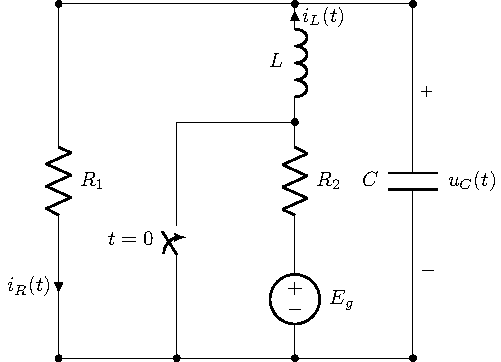
\includegraphics{figs/E2_circuito_v2.pdf}
\end{minipage}

\section*{Ejercicio 2}

En este ejercicio se analizará el comportamiento en frecuencia del circuito de la figura.


\begin{enumerate}

\item (\textbf{4p.}) Determina la función de transferencia en el dominio de Laplace
  \[
    \laplace{H} = \frac{\laplace{V_2}}{\laplace{V_1}}
  \]
  
\item (\textbf{1p.}) A partir de la expresión anterior, obtén la expresión normalizada de la función de transferencia en el dominio de la frecuencia, $\mathbf{H}(\omega)$. 

\item (\textbf{1p.}) Determina la pulsación a la que se encuentran los polos y ceros del sistema.

\item (\textbf{4p.}) Dibuja el diagrama de Bode de \textbf{amplitud y de fase}. ¿Qué tipo de filtro es este circuito?

\end{enumerate}

\begin{minipage}{0.3\textwidth}
Datos:
\begin{align*}
  C &= \SI{170}{\nano\farad}\\
  L &= \SI{30}{\milli\henry}\\
  R_L &= \SI{1}{\ohm}
\end{align*}
\end{minipage}
\begin{minipage}{0.7\textwidth}
  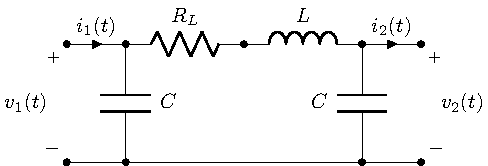
\includegraphics{figs/circuito_respuesta_frecuencia.pdf}
\end{minipage}

\section*{Ejercicio 3}

En este ejercicio se analizará el comportamiento en resonancia del circuito de la figura. Este circuito está alimentado con una fuente de tensión sinusoidal de valor eficaz $V_g = \SI{100}{\volt}$ y frecuencia $f = \SI{1}{\kilo\hertz}$. El condensador de salida tiene una capacidad de $C = \SI{50}{\nano\farad}$.

\begin{center}
  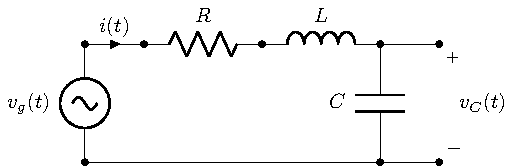
\includegraphics{figs/circuito_resonancia.pdf}
\end{center}

\begin{enumerate}

\item  (\textbf{2,5p.}) Determina la inductancia necesaria para que el circuito entre en resonancia a la frecuencia del generador.

\item  (\textbf{2,5p.}) Determina la resistencia necesaria para obtener una tensión en el condensador de $V_c = \SI{12}{\kilo\volt}$.
  
\item  (\textbf{2,5p.}) A partir de los valores de $L$ y $R$ obtenidos, determina el ancho de banda del circuito y las frecuencias de potencia mitad.

\item  (\textbf{2,5p.}) La frecuencia del generador tiene una tolerancia de $\pm1\%$. Manteniendo los valores de $L$ y $R$ obtenidos en los apartados 1 y 2, determina el valor eficaz de la corriente y la tensión en el condensador en los valores extremos de esta tolerancia.
  
\end{enumerate}

\section*{Ejercicio 4}

El circuito de la figura representa una fuente de corriente alterna sinusoidal alimentando un cuadripolo $Q_1$ que, a su vez, está conectado a una impedancia de carga. 
\begin{enumerate}
\item (\textbf{2,5p.}) Determina los parámetros impedancia del cuadripolo.
\item (\textbf{2,5p.}) A partir del resultado obtenido en el apartado anterior, calcula la impedancia de entrada del cuadripolo. A partir de este resultado, obtén la impedancia que debe tener el generador para se produzca máxima transferencia de potencia.
\item (\textbf{2,5p.}) Determina los parámetros admitancia de un cuadripolo, $Q_T$, conformado por una asociación paralelo-paralelo de dos cuadripolos $Q_1$ idénticos. Dibuja los circuitos necesarios para comprobar si existe interacción entre los cuadripolos (test de Brune), y razona el resultado que se obtendría en este caso. 
\item (\textbf{2,5p.}) ¿Cuál es la impedancia de entrada del cuadripolo $Q_T$ si en su puerto de salida tiene la misma impedancia $\overline{Z}_L$?
\end{enumerate}


\begin{minipage}{0.3\textwidth}
  Datos:
  \begin{itemize}
  \item $R$ = \SI{1}{\ohm}
  \item $X_C$ = \SI{2}{\ohm}
  \item $\overline{Z}_L$ = -j\SI{2}{\ohm}
  \end{itemize}
\end{minipage}
\begin{minipage}{0.7\textwidth}
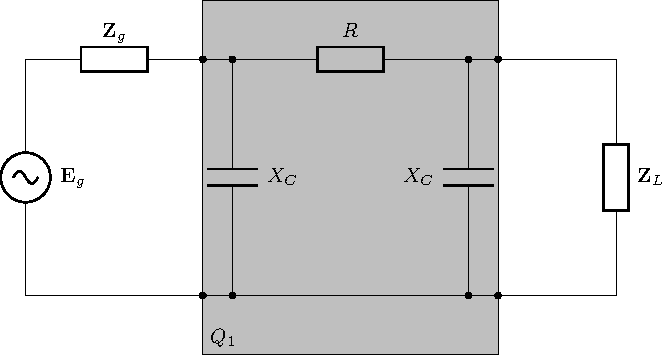
\includegraphics{figs/E5_circuito.pdf}
\end{minipage}

\end{document}

% Local Variables:
% ispell-local-dictionary: "castellano"
% End:

